\documentclass[xcolor={table}]{beamer}
\usepackage{fleqn}
%\usepackage{epsf}
\usepackage{graphicx}
\usepackage{coordsys} %for \numbline command
%\usepackage{dingbat}
%\usepackage{aima2e-slides}

%Setup appearance:

\usetheme{Darmstadt}
\usefonttheme[onlylarge]{structurebold}
\setbeamerfont*{frametitle}{size=\normalsize,series=\bfseries}
\setbeamertemplate{navigation symbols}{}
\setbeamertemplate{bibliography item}{[\theenumiv]}
\setbeamertemplate{caption}[numbered]

% Standard packages
\usepackage[english]{babel}
\usepackage[latin1]{inputenc}
\usepackage{times}
\usepackage[T1]{fontenc}
\usepackage{multirow}
\usepackage{subfigure}
\usepackage{pbox}
\usepackage{arydshln}
\usepackage{pifont}
\usepackage{cancel}

% Source Code packages
\usepackage{algorithm2e}
\usepackage{listings}

\lstset{ %
language=Octave,                % choose the language of the code
basicstyle=\footnotesize,       % the size of the fonts that are used for the code
numbers=left,                   % where to put the line-numbers
numberstyle=\footnotesize,      % the size of the fonts that are used for the line-numbers
stepnumber=1,                   % the step between two line-numbers. If it's 1 each line will be numbered
numbersep=5pt,                  % how far the line-numbers are from the code
backgroundcolor=\color{white},  % choose the background color. You must add \usepackage{color}
showspaces=false,               % show spaces adding particular underscores
showstringspaces=false,         % underline spaces within strings
showtabs=false,                 % show tabs within strings adding particular underscores
frame=single,	                % adds a frame around the code
tabsize=2,	                % sets default tabsize to 2 spaces
captionpos=b,                   % sets the caption-position to bottom
breaklines=true,                % sets automatic line breaking
breakatwhitespace=false,        % sets if automatic breaks should only happen at whitespace
escapeinside={\%*}{*)}          % if you want to add a comment within your code
}

% Setup TikZ
\usepackage{tikz}
\usetikzlibrary{arrows}
\tikzstyle{block}=[draw opacity=0.7,line width=1.4cm]

%%%%%%%%%%%%%%%%%%%%%%%%%%%%%%%%%%%%%%%%%%%%
%% Start newcommand defs taken from aima slides style file %%%%%%%%%%%%%%
%%%%%%%%%%%%%%%%%%%%%%%%%%%%%%%%%%%%%%%%%%%%

%%%%%%%%%%%% elements of programs %%%%%%%%%%%%%%%%%%%%%%%%%%%%%%%%%


\newlength{\codewidth}
\setlength{\codewidth}{\textwidth}
\addtolength{\codewidth}{-0.5in}

\newcommand{\FigBox}[1]{%%% The alternative to figbox - pnorvig
\noindent\framebox[\textwidth]{%
\begin{minipage}{\codewidth}%
#1%
\end{minipage}}%
}

\newcommand{\defprog}[1]{\txr{\mbox{{\sc #1}}}}
\newcommand{\prog}[1]{\mbox{{\sc #1}}}   %%% same as defprog
\newcommand{\noprog}[1]{\mbox{{\sc #1}}} %%% same as defprog
\newcommand{\system}[1]{\mbox{{\sc #1}}} %%% same as defprog
\newcommand{\nosystem}[1]{\mbox{{\sc #1}}} %%% same as defprog
\newcommand{\act}[1]{{\it #1}}
\newcommand{\key}[1]{\txb{{\bf #1}}}
\def\k{\key}
\newcommand{\var}[1]{\txg{{\it #1}}}
\def\v{\var}
\def\p{\prg}
\newcommand{\setq}[2]{#1\hbox{$\,\leftarrow\,$}#2}
\newcommand{\setqmath}[2]{#1 \leftarrow #2}

%%pnorvig Mar 14 1994:
\newcommand{\labl}[1]{\prog{#1}}	% Statement Label in code
\newcommand{\cmt}[1]{{\tt /*} {\it #1} {\tt */}}	% Comment in code
\newcommand{\rcmt}[1]{\hfill {\tt /*} {\it #1} {\tt */}}
\newcommand{\Endfn}[1]{}		% End of a function in code
\newcommand{\fnsep}{\hspace*{0in}\raisebox{3pt}{\rule{\codewidth}{0.2pt}}\hfill}	% Between functions in code

\def\code{\noindent\nobreak\begin{scriptsize}
        \begingroup\obeylines\obeyspaces\docode}
\def\docode#1{\noindent\framebox[\columnwidth][l]%
{~~\begin{minipage}{\codewidth}~
#1
~\end{minipage}}\endgroup%
\nobreak\end{scriptsize}\noindent\ignorespaces}
\def\asis{\obeylines\obeyspaces}
\def\ttp{.\skip -0.5em\ }
{\obeyspaces\global\def {\ }}

%% Fine tuning for perfect formatting

\newcommand{\ac}{,\hspace{0.15em}}
\newcommand{\ts}{\,}
\newcommand{\bodysep}{\vspace{0.1in}}
\newcommand{\subfnsep}{\vspace{0.06in}}
\newcommand{\prebnfsep}{\vspace{-0.25in}}
\newcommand{\postbnfsep}{\vspace{0.1in}}
\newcommand{\fnvar}[1]{\prog{#1}}
\newcommand{\func}[3]{\key{function} \defprog{#1}(\txg{#2}) \key{returns} #3}
\newcommand{\nofunc}[3]{\key{function} \noprog{#1}(#2) \key{returns} #3}
\newcommand{\proc}[2]{\key{procedure} \defprog{#1}(\txg{#2})}
\newcommand{\noproc}[2]{\key{procedure} \noprog{#1}(#2)}
\newcommand{\firstinputs}[2]{\key{inputs}: \var{#1}, #2}
\newcommand{\inputs}[2]{\phantom{\key{inputs}: }\var{#1}, #2}
\newcommand{\firstlocal}[2]{\key{local variables}: \var{#1}, #2}
\newcommand{\local}[2]{\phantom{\key{local variables}: }\var{#1}, #2}
\newcommand{\firststatic}[2]{\key{static}: \var{#1}, #2}
\newcommand{\static}[2]{\phantom{\key{static}: }\var{#1}, #2}

%%%%%%%%%%%%%%%%%%%%%%%%%%

\def\mysum{\begin{Huge}\mbox{$\Sigma$}\end{Huge}}
\def\myint{\begin{LARGE}\mbox{$\int$}\end{LARGE}}
\def\myprod{\begin{Huge}\mbox{$\Pi$}\end{Huge}}

\font\smathbold=cmbx10 scaled 1700
\newcommand{\smbf}[1]{\mbox{{\smathbold #1}}}
\newcommand{\mbf}[1]{\mbox{{\bf #1}}}

%%%%%%% Useful formatting commands for lines of text etc.
\def\tab{\hbox{\kern0.4in}}    %% Insert space (even at start of line)
\def\al{\\\tab}                %% Next line is indented
\def\nl{\\\tab\tab}            %% Next line is double-indented
\def\nnl{\\\tab\tab\tab}       %% Next line is triple-indented
%\def{$\diamondsuit\ \ $}  %% Itemization without all the spacing
\def\bull{\vskip -8pt\item{$\bullet$\ }} %% Itemization with less spacing
\def\u#1{$\underline{\mbox{#1}}$}
\def\q#1{\txm{\u{#1}??}}

%%%%%% logical symbols
\newcommand{\entails}{\models}
%\newcommand{\implies}{\:\;{\Rightarrow}\:\;}
\newcommand{\textimplies}{\;{\Rightarrow}\;}
\newcommand{\impliessymbol}{\Rightarrow}
\newcommand{\lequiv}{\;\;{\Leftrightarrow}\;\;}
\newcommand{\textlequiv}{\;{\Leftrightarrow}\;}
\newcommand{\lequivsymbol}{\Leftrightarrow}
\newcommand{\xor}{\not\lequiv}
\newcommand{\All}[1]{\forall\,#1\;\;}
\newcommand{\Exi}[1]{\exists\,#1\;\;}
\newcommand{\Exii}[1]{\exists!\,#1\;\;}% -pnorvig
\newcommand{\Iot}[2]{\iota\,#1\,#2}
\newcommand{\Lam}[2]{\lambda #1\;#2}
\newcommand{\Qua}[3]{[#1\,#2\;#3]}

\newcommand{\union}{{\,{\cup}\,}}
\newcommand{\intersection}{{\,{\cap}\,}}
\renewcommand{\emptyset}{\{\,\}}
\newcommand{\emptylist}{[\,]}
\newcommand{\adjoin}[2]{\{#1|#2\}}
\newcommand{\elt}{{\,{\in}\,}}  %%%cuts down on spacing
\newcommand{\eq}{{\,{=}\,}}  %%%cuts down on spacing
\def\stimes{{\,\times\,}}       %%%cuts down on spacing


%%%%%%% Formatting tables - AIMA uses full-width tables with spacing

\newenvironment{mytabular}%
{\noindent\begin{tabular*}{\textwidth}}%
{\end{tabular*}}

\newcommand{\tabtop}{\rule{0pt}{2ex}}%%Use after hline in body of table
\newcommand{\tabbot}{\rule[-1ex]{0pt}{1.8ex}}%%Use before hline " " " "
\newcommand{\tabhead}{\rule[-0.85ex]{0pt}{2.8ex}}%%Use in lines between hlines
\newcommand{\squad}{\hspace*{0.5em}}%%Use occasionally at left edge
\newcommand{\sq}[1]{\hspace*{#1\textwidth}}
\def\tf{\rm} %% table font


\def\<{\langle}
\def\>{\rangle}

%\usepackage[dvips]{color}
\definecolor{myred}{rgb}{0.7,0.0,0.0}
\definecolor{myblue}{rgb}{0.0,0.0,0.5}
\definecolor{mygreen}{rgb}{0.0,0.3,0.0}

\newcommand{\txr}[1]{\textcolor{myred}{#1}}
\newcommand{\txR}[1]{\textcolor{red}{#1}}
\newcommand{\txb}[1]{\textcolor{myblue}{#1}}
\newcommand{\txg}[1]{\textcolor{mygreen}{#1}}
\newcommand{\txm}[1]{\textcolor{magenta}{#1}}

\newcommand{\mat}[1]{\textcolor{myred}{#1}}
\newcommand{\defn}[1]{\textcolor{myblue}{#1}}
\newcommand{\mynote}[1]{\textcolor{mygreen}{#1}}


\newcommand{\sr}[1]{\mathrel{\raisebox{-0.6ex}{$\stackrel{#1}{\longrightarrow}$}}}
\newcommand{\srbox}[1]{\sr{\fboxsep=1pt\fbox{$\,{\scriptstyle #1}\,$}}}
\newcommand{\srboxbox}[1]{\sr{\fboxsep=1pt\fbox{\fbox{$\,{\scriptstyle #1}\,$}}}}

\def\Diff{\mbox{{\it Diff}}}

%%%%%% probability and decision theory
\newcommand{\pv}{\mbf{P}}
\newcommand{\qv}{\mbf{Q}}
\newcommand{\given}{\mid}
\def\transition#1#2{q(#1\rightarrow #2)}
\newcommand{\otherthan}{\overline}
\newcommand{\Parents}{Parents}
\newcommand{\parents}{parents}
\newcommand{\Children}{Children}
\newcommand{\children}{children}
\newcommand{\MarkovBlanket}{MB}
\newcommand{\markovBlanket}{mb}


\def\X{\mbf{X}}
\def\x{\mbf{x}}
\def\sx{\smbf{x}}
\def\Y{\mbf{Y}}
\def\y{\mbf{y}}
\def\sy{\smbf{y}}
\def\E{\mbf{E}}
\def\e{\mbf{e}}
\def\D{\mbf{D}}
\def\d{\mbf{d}}
\def\sbe{\smbf{e}}
\def\sE{\smbf{E}}
\def\T{\mbf{T}}
\def\O{\mbf{O}}
\def\se{\smbf{e}}
\def\Z{\mbf{Z}}
\def\z{\mbf{z}}
\def\sz{\smbf{z}}
\def\F{\mbf{F}}
\def\f{\mbf{f}}
\def\A{\mbf{A}}
\def\B{\mbf{B}}
\def\C{\mbf{C}}
\def\b{\mbf{b}}
\def\m{\mbf{m}}
\def\I{\mbf{I}}
\def\H{\mbf{H}}
\def\zeroes{\mbf{0}}
\def\ones{\mbf{1}}
\def\ev{\mbf{ev}}
\def\fv{\mbf{ev}}
\def\sv{\mbf{sv}}

\usepackage{rotating} % for sideways headings

%\usepackage{listings}
%\usepackage{xfrac} % for slanted fractions using sfrac
%
%% the answer environment
%\usepackage{verbatim}   % for the comment environment
%\usepackage{ifthen}
%\usepackage{lipsum}
%\newenvironment{answer}%
%        {%
%            \ifthenelse{\isundefined{\showanswer}}%
%                    {\expandafter\comment}%
%                    {~\\ \noindent\rule{\textwidth}{0.4pt}}%
%                    }%
%         {%
%            \ifthenelse{\isundefined{\showanswer}}%
%                    {\expandafter\endcomment}%
%                    {~\\ \noindent\rule{\textwidth}{0.4pt} \newpage}%
%          }
%
%\usepackage{arydshln}
%\usepackage{capt-of}

\DeclareSymbolFont{extraup}{U}{zavm}{m}{n}
\DeclareMathSymbol{\varclub}{\mathalpha}{extraup}{84}
\DeclareMathSymbol{\varspade}{\mathalpha}{extraup}{85}
\DeclareMathSymbol{\varheart}{\mathalpha}{extraup}{86}
\DeclareMathSymbol{\vardiamond}{\mathalpha}{extraup}{87}

%%%%%%%%%%%%%%%%%%%%%%%%%%%%%%%%%%%%%%%%%%%%
%% End newcommand defs taken from aima slides style file %%%%%%%%%%%%%%
%%%%%%%%%%%%%%%%%%%%%%%%%%%%%%%%%%%%%%%%%%%%

\usepackage{xifthen}% provides \isempty test

\urlstyle{same} %ensure that urls are formatted in the same font as other text

% tikz sert up for MDP diagrams
%\usepackage{tikz}			% for MDP dfiagrams
%\usetikzlibrary{positioning,angles,quotes}
\usepackage{pgfplots}         % it load tikz too
%\pgfplotsset{compat=1.16}
\pgfplotsset{compat=1.14}
\usetikzlibrary{automata,
                arrows.meta,    %   ...customizing arrows
                positioning,    %   ...positioning nodes
                quotes}         % For edge labels
\usepgfplotslibrary{fillbetween}


%To get Table, Figure, Equation Numbers to work!
\usepackage{xr}
\externaldocument{FMLPDA2-Main-NewMathTemplate}
%To get nice labeled matrices in  MDB examples
\usepackage{kbordermatrix}
 % For vertical alignment in table cells
\usepackage[export]{adjustbox}
% For citet and citep commands
\usepackage[round]{natbib}

%Use tikz package and command is used to put circles around symbols inline useful for NN examples
\newcommand*\circled[1]{\tikz[baseline=(char.base)]{
            \node[shape=circle,draw,inner sep=2pt,minimum size=20pt] (char) {#1};}}

%%% This section command that adds a big page with section dividers
\usepackage{xifthen}% provides \isempty test
\newcommand{\SectionSlide}[2][]{
	\ifthenelse{\isempty{#1}}
		{\section{#2}\begin{frame} \begin{center}\begin{huge}#2\end{huge}\end{center}\end{frame}}
		{\section[#1]{#2}\begin{frame} \begin{center}\begin{huge}#2\end{huge}\end{center}\end{frame}}
}
%Extends the section slide to to include a shortened section title for the navigation bar as a second parameter
\newcommand{\SectionSlideShortHeader}[3][]{
	\ifthenelse{\isempty{#1}}
		{\section[#3]{#2}\begin{frame} \begin{center}\begin{huge}#2\end{huge}\end{center}\end{frame}}
		{\section[#1]{#2}\begin{frame} \begin{center}\begin{huge}#3\end{huge}\end{center}\end{frame}}
}



\newcommand{\Toprule}[0]{\hline}
\newcommand{\Midrule}[0]{\hline}
\newcommand{\Botrule}[0]{\hline}
\DeclareMathOperator*{\argmax}{arg\,max}
\DeclareMathOperator*{\argmin}{arg\,min}

\newcommand{\keyword}[1]{{\textbf{#1}}\index{#1}}
\newcommand{\indexkeyword}[1]{#1\index{#1}}
\newcommand{\keywordDef}[1]{{\textbf{#1}}\index{#1|textbf}}
\newcommand{\indexkeywordDef}[1]{{#1}\index{#1|textbf}}
\newcommand{\keywordAlias}[2]{{\textbf{#1}}\index{#2}}
\newcommand{\indexkeywordAlias}[2]{#1\index{#2}}
\newcommand{\keywordDefAlias}[2]{{\textbf{#1}}\index{#2|textbf}}
\newcommand{\indexkeywordDefAlias}[2]{{#1}\index{#2|textbf}}
\newcommand{\keywordCR}[2]{{\textbf{#1}}\index{#1|see {#2}}}
\newcommand{\keywordCRAlias}[3]{{\textbf{#1}}\index{#2|see {#3}}}
\newcommand{\indexkeywordCR}[2]{#1\index{#1|see {#2}}}
\newcommand{\indexkeywordCRAlias}[3]{#1\index{#2|see {#3}}}
\newcommand{\mightdo}[1]{}
\newcommand{\featN}[1]{\textsc{#1}}
\newcommand{\featL}[1]{\textit{#1}}
 \newcommand{\ourRef}[1]{\ref{#1}$^{\text{\tiny[\pageref{#1}]}}$}
 \newcommand{\ourEqRef}[1]{\eqref{#1}$^{\text{\tiny[\pageref{#1}]}}$}
 \newcommand{\ourItemExtra}{\item[\raisebox{0.25ex}{$\mathbf{\Asterisk}$} \addtocounter{enumi}{1}\arabic{enumi}.]} 
 \newcommand{\rlState}[1]{\textsc{#1}} % Used in reinforcement learning chapter
\newcommand{\rlAction}[1]{\textit{#1}} % Used in reinforcement learning chapter

\title{Information-based Learning}
\subtitle{Sections $4.4, 4.5$}
	\author{John D. Kelleher and Brian Mac Namee and Aoife D'Arcy}
	\date{}
		
\begin{document}
\begin{frame}
	\titlepage
\end{frame}
\begin{frame}
	 \tableofcontents
\end{frame}

\SectionSlideShortHeader{Alternative Feature Selection Metrics}{Feature Selection}

 \begin{frame} 
\begin{itemize}
	\item Entropy based information gain, preferences features with many values. 
	\item One way of addressing this issue is to use \keyword{information gain ratio} which is computed by dividing the information gain of a feature by the amount of information used to determine the value of the feature:
\end{itemize}
\begin{equation}
GR\left(d,\mathcal{D}\right) = \frac{IG\left(d,\mathcal{D}\right)}{- \displaystyle \sum_{l \in levels\left(d\right)} \left(P(d=l) \times log_2(P(d=l)) \right)}
\label{eq:infogainratio}
\end{equation}
\end{frame} 


 \begin{frame} 
\begin{eqnarray*}
IG\left(\featN{Stream},\mathcal{D}\right)& = &0.3060  \\
IG\left(\featN{Slope},\mathcal{D}\right)& =& 0.5774 \\
IG\left(\featN{Elevation},\mathcal{D}\right)& =& 0.8774 \\
\end{eqnarray*}
\end{frame} 



 \begin{frame} 
 \begin{tiny}
\begin{equation*}
	\begin{alignedat}{2}
&H\left(\featN{Stream},\mathcal{D}\right)\\
&= - \sum_{l \in  \left\{ \begin{subarray}{1} \featL{true}, \\ \featL{false} \end{subarray} \right\}} P(\featN{Stream}=l) \times log_2\left(P(\featN{Stream}=l)\right)\\
		&= -\left( \left( ^4/_7 \times log_2( ^4/_7) \right) + \left( ^3/_7  \times log_2(^3/_7)\right) \right)\\
		&= 0.9852~bits \\
		~ & \\
&H\left(\featN{Slope},\mathcal{D}\right)\\
&= - \sum_{l \in  \left\{ \begin{subarray}{1} \featL{flat}, \\ \featL{moderate}, \\ \featL{steep} \end{subarray} \right\}} P(\featN{Slope}=l) \times log_2\left(P(\featN{Slope}=l)\right)\\
		&= -\left( \left( ^1/_7 \times log_2( ^1/_7) \right) + \left( ^1/_7  \times log_2(^1/_7)\right) + \left( ^5/_7  \times log_2(^5/_7)\right) \right)\\
		&= 1.1488~bits \\
				~ & \\
&H\left(\featN{Elevation},\mathcal{D}\right)\\
&= - \sum_{l \in  \left\{ \begin{subarray}{1} \featL{low}, \\ \featL{medium}, \\ \featL{high}, \\ \featL{highest} \end{subarray} \right\}} P(\featN{Elevation}=l) \times log_2\left(P(\featN{Elevation}=l)\right)\\
		&= -\left( \left( ^1/_7 \times log_2( ^1/_7) \right) + \left( ^2/_7  \times log_2(^2/_7)\right) + \left( ^3/_7  \times log_2(^3/_7)\right) + \left( ^1/_7  \times log_2(^1/_7)\right)\right)\\
		&= 1.8424~bits
	\end{alignedat}
\end{equation*}
\end{tiny}
\end{frame} 



 \begin{frame} 
\begin{equation*}
	\begin{alignedat}{2}
	GR\left(\featN{Stream},\mathcal{D}\right) & = \frac{0.3060}{0.9852} = 0.3106 \\
	GR\left(\featN{Slope},\mathcal{D}\right) & = \frac{0.5774}{1.1488} = 0.5026 \\
	GR\left(\featN{Elevation},\mathcal{D}\right) & = \frac{0.8774}{1.8424} = 0.4762 \\
	\end{alignedat}
\end{equation*}
\end{frame} 

 \begin{frame} 
\begin{figure}
\centerline{
	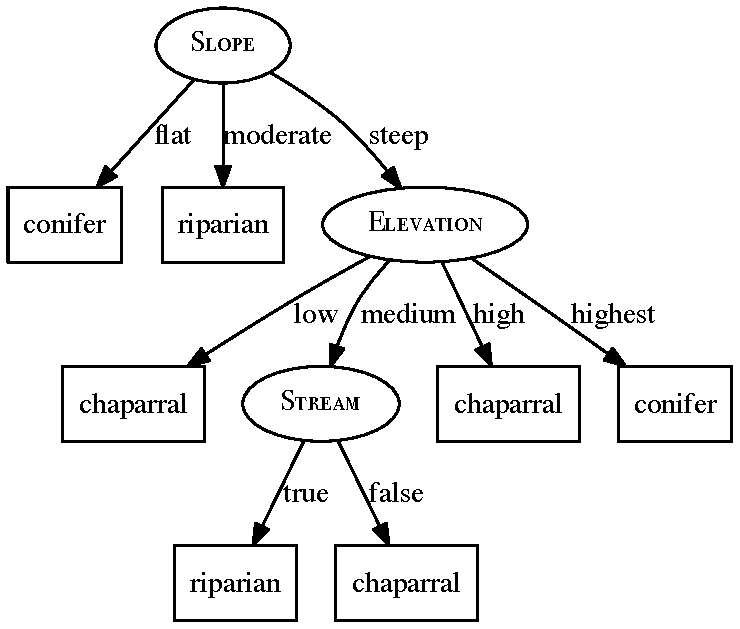
\includegraphics[width=0.8\textwidth]{./images/ex-hand-ecology-dectree5_mod.pdf}
}
\caption{The vegetation classification decision tree generated using information gain ratio.}
\label{fig:ex-hand-dectree5}
\end{figure}
\end{frame} 

 \begin{frame} 
\begin{itemize}
	\item Another commonly used measure of impurity is the \keyword{Gini index}:
\end{itemize}
\begin{equation}
Gini\left(t,\mathcal{D}\right) = 1 - \sum_{l \in levels(t)} P(t=l)^2
\label{eq:gini}
\end{equation}
\begin{itemize}
	\item  The Gini index can be thought of as calculating how often you would misclassify an instance in the dataset if you classified it based on the distribution of classifications in the dataset. 
	\item Information gain can be calculated using the Gini index by replacing the entropy measure with the Gini index.
\end{itemize}
\end{frame} 

 \begin{frame} 
\begin{equation*}
	\begin{alignedat}{2}
&Gini\left(\featN{Vegetation},\mathcal{D}\right)\\
&= 1 - \sum_{l \in  \left\{ \begin{subarray}{1} \featL{chapparal}, \\ \featL{riparian}, \\ \featL{conifer} \end{subarray} \right\}} P(\featN{Vegetation}=l)^2\\
		&= 1- \left( \left(3/_7\right)^2 + \left( ^2/_7\right)^2 + \left( ^2/_7\right)^2 \right)\\
		&= 0.6531
	\end{alignedat}
\end{equation*}
\end{frame} 

 \begin{frame} 
\begin{table}
\caption{Partition sets (Part.), entropy, Gini index, remainder (Rem.), and information gain (Info. Gain) by feature}
\label{tab:giniindexsplits}
\centering
\begin{scriptsize}
\begin{tabular}{ccccccc}
\hline
Split by &  &              &  & Partition &  & Info.\\
Feature & Level & Part.  & Instances & Gini Index & Rem. & Gain\\
\hline
\multirow{2}{*}{\featN{Stream}} & \featL{true} & $\mathcal{D}_1$  & $\mathbf{d}_2,\mathbf{d}_3,\mathbf{d}_6,\mathbf{d}_7$ & 0.625 & \multirow{2}{*}{0.5476} & \multirow{2}{*}{0.1054}\\
 & \featL{false} & $\mathcal{D}_2$ & $\mathbf{d}_1,\mathbf{d}_4,\mathbf{d}_5$ & 0.4444 &  & \\
\hline

\multirow{3}{*}{\featN{Slope}} & \featL{flat} & $\mathcal{D}_3$ & $\mathbf{d}_5$  & 0 & \multirow{3}{*}{0.4} & \multirow{3}{*}{0.2531}\\
& \featL{moderate} & $\mathcal{D}_4$ & $\mathbf{d}_2$ & 0 &  & \\
& \featL{steep} & $\mathcal{D}_5$ & $\mathbf{d}_1,\mathbf{d}_3,\mathbf{d}_4,\mathbf{d}_6,\mathbf{d}_7$ & 0.56 &  & \\

\hline
\multirow{4}{*}{\featN{Elevation}} & \featL{low} & $\mathcal{D}_6$ & $\mathbf{d}_2$  & 0 & \multirow{4}{*}{0.3333} & \multirow{4}{*}{0.3198}\\
 & \featL{medium} & $\mathcal{D}_7$ & $\mathbf{d}_3,\mathbf{d}_4$ & 0.5 &  & \\
 & \featL{high} & $\mathcal{D}_8$ & $\mathbf{d}_1,\mathbf{d}_5,\mathbf{d}_7$ & 0.4444 &  & \\
 & \featL{highest} & $\mathcal{D}_9$ & $\mathbf{d}_6$ & 0 &  & \\
\hline
\end{tabular}
\end{scriptsize}
\end{table}
\end{frame} 

\SectionSlideShortHeader{Handling Continuous Descriptive Features}{Cont. Desc. Features}

\begin{frame}
	\begin{itemize}
	\item The easiest way to handle continuous valued descriptive features is to turn them into boolean features by defining a threshold  and using this threshold to partition the instances based their value of the continuous  descriptive feature.
	\item How do we set the threshold?
	\end{itemize}
\end{frame}

\begin{frame}
	\begin{enumerate}
	\item The instances in the dataset are sorted according to the continuous feature values. 
	\item The adjacent instances in the ordering that have different classifications are then selected as possible threshold points. 
	\item The optimal threshold is found by computing the information gain for each of these classification transition boundaries and selecting the boundary with the highest information gain as the threshold. 
	\end{enumerate}
\end{frame}

\begin{frame}
	\begin{itemize}
		\item Once a threshold has been set the dynamically created new boolean feature can compete with the other categorical features for selection as the splitting feature at that node.
		\item This process can be repeated at each node as the tree grows.
	\end{itemize}
\end{frame}

 \begin{frame} 
\begin{table}[h]
\caption{Dataset for predicting the vegetation in an area with a continuous \featN{Elevation} feature (measured in feet).}
\label{tab:ecologydatanumeric}
\centering
\begin{footnotesize}
\begin{tabular}{c c c r c }
\hline
\featN{ID}	 & \featN{Stream}	& \featN{Slope} & \featN{Elevation} & \featN{Vegetation}\\
\hline
1 & false & steep & 3\,900 & chapparal\\
2 & true & moderate & 300 & riparian\\
3 & true & steep & 1\,500 & riparian\\
4 & false & steep & 1\,200 & chapparal\\
5 & false & flat & 4\,450 & conifer\\
6 & true & steep & 5\,000 & conifer\\
7 & true & steep & 3\,000 & chapparal\\
\hline
\end{tabular}
\end{footnotesize}
\end{table}
\end{frame} 



 \begin{frame} 
\begin{table}[h]
\caption{Dataset for predicting the vegetation in an area sorted by the continuous \featN{Elevation} feature.}
\label{tab:ecologydatanumericsorted}
\centering
\begin{footnotesize}
\begin{tabular}{c c c r c }
\hline
\featN{ID}	 & \featN{Stream}	& \featN{Slope} & \featN{Elevation} & \featN{Vegetation}\\
\hline
2 & true & moderate & 300 & riparian\\
4 & false & steep & 1\,200 & chapparal\\
3 & true & steep & 1\,500 & riparian\\
7 & true & steep & 3\,000 & chapparal\\
1 & false & steep & 3\,900 & chapparal\\
5 & false & flat & 4\,450 & conifer\\
6 & true & steep & 5\,000 & conifer\\
\hline
\end{tabular}
\end{footnotesize}
\end{table}
\end{frame} 



 \begin{frame} 
\begin{table}[htb]
\caption{Partition sets (Part.), entropy, remainder (Rem.), and information gain (Info. Gain) for the candidate \featN{Elevation} thresholds: $\geq$$750$, $\geq$$1\,350$, $\geq$$2\,250$ and $\geq$$4\,175$.}
\label{tab:cont-feat-split1}
\centering
\begin{footnotesize}
\resizebox{\textwidth}{!}{
\begin{tabular}{cccccc}
\hline
Split by &              &  & Partition &  & Info.\\
Threshold & Part.  & Instances & Entropy & Rem. & Gain \\
\hline
\multirow{2}{*}{$\geq$$750$} & $\mathcal{D}_1$  & $\mathbf{d}_2$ & 0.0 & \multirow{2}{*}{1.2507} & \multirow{2}{*}{0.3060}\\
 & $\mathcal{D}_2$ & $\mathbf{d}_4,\mathbf{d}_3,\mathbf{d}_7,\mathbf{d}_1,\mathbf{d}_5,\mathbf{d}_6$ & 1.4591 &  & \\
\hline
\multirow{2}{*}{$\geq$$1\,350$} & $\mathcal{D}_3$  & $\mathbf{d}_2,\mathbf{d}_4$ & 1.0 & \multirow{2}{*}{1.3728} & \multirow{2}{*}{0.1839}\\
 & $\mathcal{D}_4$ & $\mathbf{d}_3,\mathbf{d}_7,\mathbf{d}_1,\mathbf{d}_5,\mathbf{d}_6$ & 1.5219 &  & \\
\hline
\multirow{2}{*}{$\geq$$2\,250$} & $\mathcal{D}_5$  & $\mathbf{d}_2,\mathbf{d}_4,\mathbf{d}_3$ & 0.9183 & \multirow{2}{*}{0.9650} & \multirow{2}{*}{0.5917}\\
 & $\mathcal{D}_6$ & $\mathbf{d}_7,\mathbf{d}_1,\mathbf{d}_5,\mathbf{d}_6$ & 1.0 &  & \\
\hline
\multirow{2}{*}{$\geq$$4\,175$} & $\mathcal{D}_7$ & $\mathbf{d}_2,\mathbf{d}_4,\mathbf{d}_3,\mathbf{d}_7,\mathbf{d}_1$ & 0.9710 & \multirow{2}{*}{0.6935} & \multirow{2}{*}{0.8631}\\
& $\mathcal{D}_8$ & $\mathbf{d}_5,\mathbf{d}_6$ & 0.0 &  & \\
\hline
\end{tabular}
}
\end{footnotesize}
\end{table}
\end{frame} 



 \begin{frame} 
\begin{figure}
\centerline{
	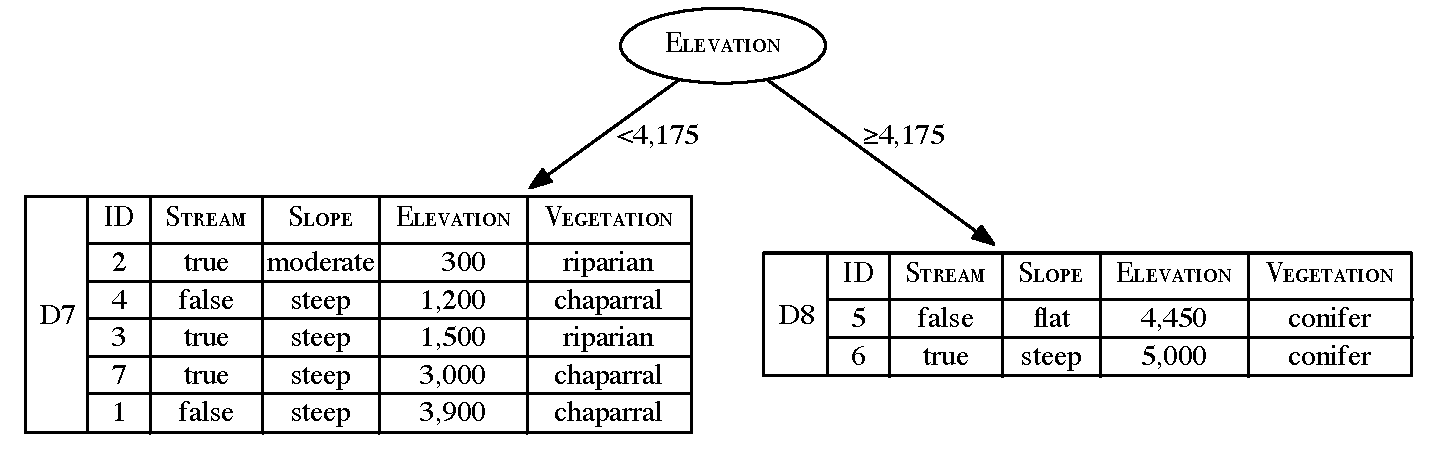
\includegraphics[width=\textwidth]{./images/ex-hand-ecology-dectree6_mod.pdf}
}
\caption{The vegetation classification decision tree after the dataset has been split using \featN{Elevation}~$\geq4\,175$.}
\label{fig:ex-hand-dectree6}
\end{figure}
\end{frame} 

 \begin{frame} 
\begin{figure}
\centerline{
	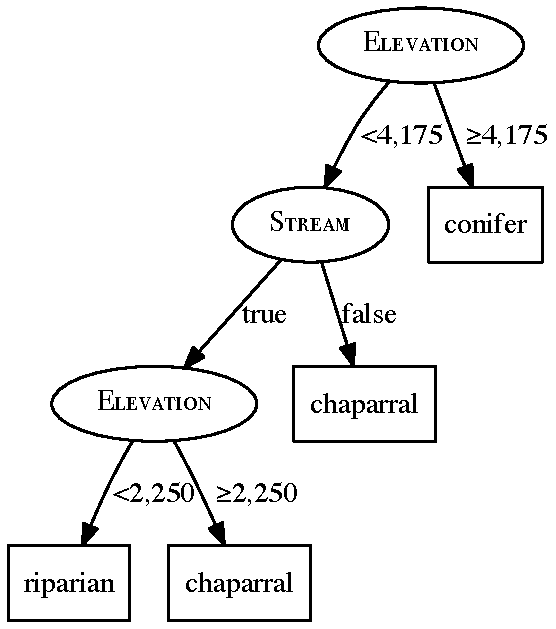
\includegraphics[width=0.5\textwidth]{./images/ex-hand-ecology-dectree7_mod.pdf}
}
\caption{The decision tree that would be generated for the vegetation classification dataset listed in Table \ourRef{tab:ecologydatanumericsorted} using information gain.}
\label{fig:ex-hand-dectree7}
\end{figure}
\end{frame} 


\SectionSlideShortHeader{Predicting Continuous Targets}{Cont. Targets}

\begin{frame}
		\begin{itemize}
\item Regression trees are constructed so as to reduce the \defn{variance} in the set of training examples at each of the leaf nodes in the tree
\item We can do this by adapting the ID3 algorithm to use a measure of variance rather than a measure of classification impurity (entropy) when selecting the best attribute
		\end{itemize}
\end{frame}

 \begin{frame} 
		\begin{itemize}
		\item The impurity (variance) at a node can be calculated using the following equation:
		\end{itemize}
\begin{equation}
var\left(t, \mathcal{D}\right) = \frac{\sum_{i=1}^n \left( t_i - \bar{t}\right)^2}{n-1}
\label{eq:decvariance}
\end{equation}
		\begin{itemize}
		\item We select the feature to split on at a node by selecting the feature that minimizes the weighted variance across the resulting partitions:
		\end{itemize}
\begin{equation}
\mathbf{d}[best] = \argmin_{d \in \mathbf{d}} \sum_{l \in levels(d)} \frac{|\mathcal{D}_{d=l}|}{|\mathcal{D}|} \times var(t, \mathcal{D}_{d=l})
\label{eq:dbestselection}
\end{equation}
\end{frame} 

\begin{frame} 
\begin{figure}
\subfigure[]{\label{fig:numberlinesTarget} 
\resizebox{0.95\textwidth}{!}{\begin{picture}(310,20)(-180,-5)
\numbline*{-155}{155}
\put(-130,0){\circle*{6}}
\put(-115,0){\circle*{6}}
\put(-105,0){\circle*{6}}
\put(70,0){\circle*{6}}
\put(80,0){\circle*{6}}
\put(90,0){\circle*{6}}
\put(100,0){\circle*{6}}
\put(140,0){\sethlabel{Target}}
\end{picture} 
}
}
\subfigure[]{\label{fig:numberlinesUnderfitting}
\resizebox{0.95\textwidth}{!}{\begin{picture}(310,20)(-180,-5)
\numbline*{-155}{155}
\put(-130,0){\circle*{6}}
\put(-115,0){\circle*{6}}
\put(-105,0){\circle*{6}}
\put(70,0){\circle*{6}}
\put(80,0){\circle*{6}}
\put(90,0){\circle*{6}}
\put(100,0){\circle*{6}}
\put(140,0){\sethlabel{Underfitting}}
\qbezier(-135,0)(-133,10)(-125,10)
\qbezier(-135,0)(-133,-10)(-125,-10)
\qbezier(-125,10)(0,10)(95,10)
\qbezier(-125,-10)(0,-10)(95,-10)
\qbezier(95,10)(103,10)(105,0)
\qbezier(95,-10)(103,-10)(105,0)
\end{picture} 
}
}
\subfigure[]{\label{fig:numberlinesGoldilocks}
\resizebox{0.95\textwidth}{!}{\begin{picture}(310,20)(-180,-5)
\numbline*{-155}{155}
\put(-130,0){\circle*{6}}
\put(-115,0){\circle*{6}}
\put(-105,0){\circle*{6}}
\put(70,0){\circle*{6}}
\put(80,0){\circle*{6}}
\put(90,0){\circle*{6}}
\put(100,0){\circle*{6}}
\put(140,0){\sethlabel{Goldilocks}}
\qbezier(-135,0)(-133,10)(-125,10)
\qbezier(-135,0)(-133,-10)(-125,-10)
\qbezier(-125,10)(-115,10)(-110,10)
\qbezier(-125,-10)(-115,-10)(-110,-10)
\qbezier(-110,10)(-102,10)(-100,0)
\qbezier(-110,-10)(-102,-10)(-100,0)
\qbezier(65,0)(67,10)(75,10)
\qbezier(65,0)(67,-10)(75,-10)
\qbezier(75,10)(85,10)(95,10)
\qbezier(75,-10)(85,-10)(95,-10)
\qbezier(95,10)(103,10)(105,0)
\qbezier(95,-10)(103,-10)(105,0)
\end{picture} 
}
}
\subfigure[]{\label{fig:numberlinesOverfitting}
\resizebox{0.95\textwidth}{!}{\begin{picture}(310,20)(-180,-5)
\numbline*{-155}{155}
\put(-130,0){\circle*{6}}
\put(-115,0){\circle*{6}}
\put(-105,0){\circle*{6}}
\put(70,0){\circle*{6}}
\put(80,0){\circle*{6}}
\put(90,0){\circle*{6}}
\put(100,0){\circle*{6}}
\put(140,0){\sethlabel{Overfitting}}
\put(-130,0){\circle{9}}
\put(-115,0){\circle{9}}
\put(-105,0){\circle{9}}
\put(70,0){\circle{9}}
\put(80,0){\circle{9}}
\put(90,0){\circle{9}}
\put(100,0){\circle{9}}
\end{picture} 
}
}
\caption{(a) A set of instances on a continuous number line;  (b), (c), and (d) depict some of the potential groupings that could be applied to these instances.}
\label{fig:numberlines}
\end{figure}
\end{frame} 

\begin{frame} 
\begin{table}[htb]
\caption{A dataset listing the number of bike rentals per day.}
\label{tab:cont-target}
\centering
\begin{tiny}
\resizebox{\textwidth}{!}{\begin{tabular}{cc}
		\hline
			\begin{minipage}{0.48\textwidth}
\center{
				\begin{tabular}{ c c c r }
\featN{ID}	 & \featN{Season} & \featN{Work Day} &  \featN{Rentals}\\
\hline
1 & winter & false & 800\\ 
2 & winter & false & 826\\ 
3 & winter & true & 900\\ 
4 & spring & false & 2\,100\\ 
5 & spring & true & 4\,740\\ 
6 & spring & true & 4\,900\\ 
\hline
\end{tabular}
 }
			\end{minipage}
			&
			\begin{minipage}{0.48\textwidth}
\center{
				\begin{tabular}{ c c c r }
\featN{ID}	 & \featN{Season} & \featN{Work Day} &  \featN{Rentals}\\
\hline
7 & summer & false & 3\,000\\ 
8 & summer & true & 5\,800\\ 
9 & summer & true & 6\,200\\ 
10 & autumn & false & 2\,910\\ 
11 & autumn & false & 2\,880\\ 
12 & autumn & true & 2\,820\\
\hline
\end{tabular}
}
			\end{minipage}\\
\end{tabular}}
\end{tiny}
\end{table}
\end{frame} 



 \begin{frame} 
\begin{table}
\caption{The partitioning of the dataset in Table \ourRef{tab:cont-target} based on \featN{Season} and \featN{Work Day} features and the computation of the weighted variance for each partitioning.}
\label{tab:splits-cont}
\centering
\begin{footnotesize}
\resizebox{\textwidth}{!}{
\begin{tabular}{ccccrrr}
\hline
Split by &  &                &                  &     \multirow{2}{*}{$ \displaystyle\frac{|\mathcal{D}_{d=l}|}{|\mathcal{D}|}$}       &                                    &  Weighted                           \\
Feature   & Level      & Part.  & Instances &     & $var\left(t, \mathcal{D}\right)$ & Variance\\
\hline
\multirow{4}{*}{\featN{Season}} & \featL{winter} & $\mathcal{D}_1$  & $\mathbf{d}_1,\mathbf{d}_2,\mathbf{d}_3$  &   0.25    &  $2\,692~~$  & \multirow{4}{*}{$1\,379\,331\frac{1}{3}$}\\
                            & \featL{spring} & $\mathcal{D}_2$  & $\mathbf{d}_4,\mathbf{d}_5,\mathbf{d}_6$   &    0.25   &  $2\,472\,533\frac{1}{3}$  &                                      \\
                            & \featL{summer} & $\mathcal{D}_3$  & $\mathbf{d}_7,\mathbf{d}_8,\mathbf{d}_9$   &    0.25   &  $3\,040\,000~~$  &                                      \\
                            & \featL{autumn} & $\mathcal{D}_4$  & $\mathbf{d}_{10},\mathbf{d}_{11},\mathbf{d}_{12}$   &    0.25   &  $2\,100~~$  &                                      \\

\hline
\multirow{2}{*}{\featN{Work Day}} & \featL{true} & $\mathcal{D}_5$  & $\mathbf{d}_3,\mathbf{d}_5,\mathbf{d}_6,\mathbf{d}_{8},\mathbf{d}_{9},\mathbf{d}_{12}$      &    0.50   &  $4\,026\,346\frac{1}{3}$ & \multirow{2}{*}{$2\,551\,813\frac{1}{3}$}\\
                            & \featL{false} & $\mathcal{D}_6$  & $\mathbf{d}_1,\mathbf{d}_2,\mathbf{d}_4,\mathbf{d}_{7},\mathbf{d}_{10},\mathbf{d}_{11}$     &     0.50  &   $1\,077\,280~~$ &                                       \\
\hline
\end{tabular}
}
\end{footnotesize}
\end{table}
\end{frame} 



 \begin{frame} 
\begin{figure}
\centerline{
	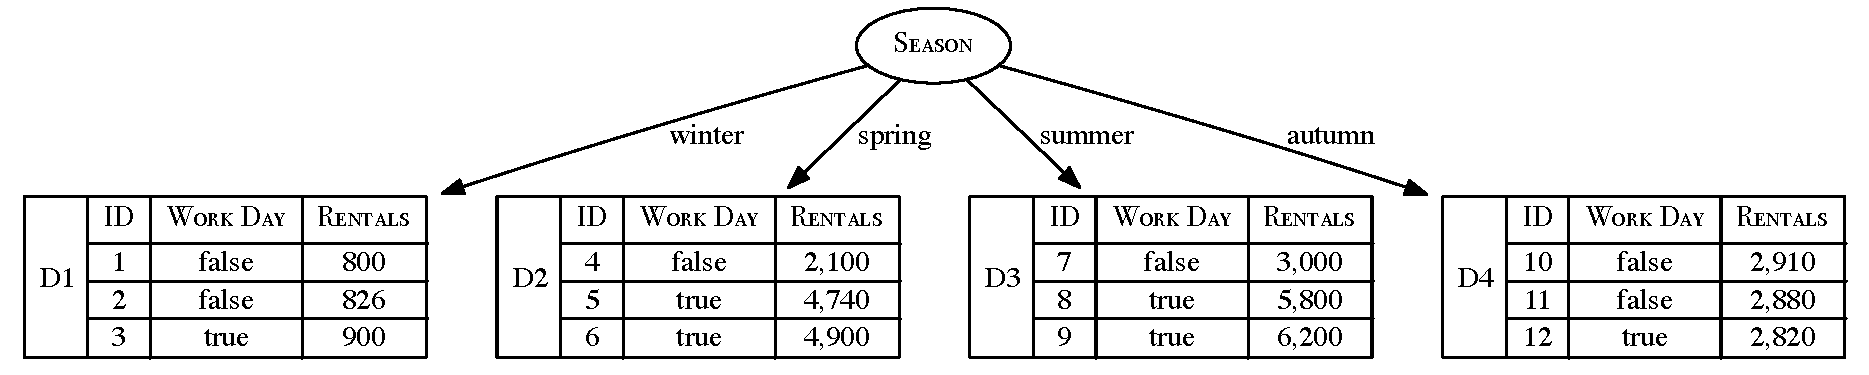
\includegraphics[width=\textwidth]{./images/ex-hand-id3-regression1_mod.pdf}
}
\caption{The decision tree resulting from splitting the data in Table \ourRef{tab:cont-target} using the feature \featN{Season}.}
\label{fig:ex-id3-regression-1}
\end{figure}
\end{frame} 



 \begin{frame} 
\begin{figure}
\centerline{
	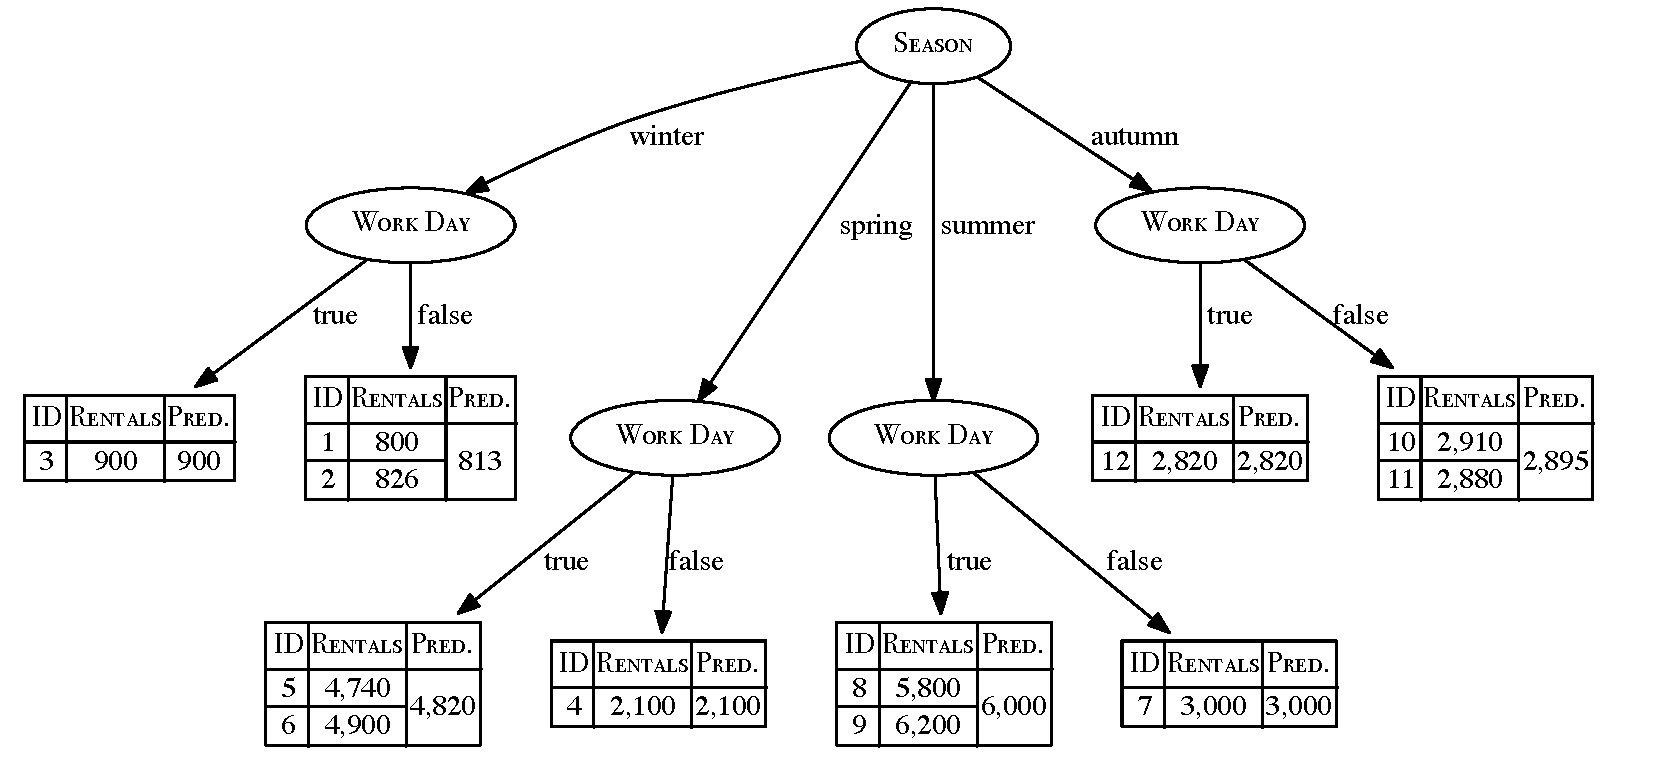
\includegraphics[width=\textwidth]{./images/ex-hand-id3-regression-final_mod.pdf}
}
\caption{The final decision tree induced from the dataset in Table \ourRef{tab:cont-target}. To illustrate how the tree generates predictions, this tree lists the instances that ended up at each leaf node and the prediction (PRED.) made by each leaf node.}
\label{fig:ex-id3-regression-final}
\end{figure}
\end{frame} 


\SectionSlideShortHeader{Noisy Data, Overfitting and Tree Pruning}{Noise and Overfitting}

\begin{frame}
	\begin{itemize}
		\item In the case of a decision tree, over-fitting involves splitting the data on an irrelevant feature. 
	\end{itemize}
\begin{block}{}
The likelihood of over-fitting occurring increases as a tree gets deeper because the resulting classifications are based on smaller and smaller subsets as the dataset is partitioned after each feature test in the path.
\end{block}
\end{frame}


\begin{frame}
\begin{itemize}
	\item \keyword{Pre-pruning}: stop the recursive partitioning early. Pre-pruning is also known as \keyword{forward pruning}.
	\begin{block}{Common \alert{Pre}-pruning Approaches}
	\begin{enumerate}
\item \keyword{early stopping}
\item \keyword{$\chi^2$ pruning} 
	\end{enumerate}
	\end{block}
	\item \keyword{Post-pruning}: allow the algorithm to grow the tree as much as it likes and then prune the tree of the branches that cause over-fitting.
\end{itemize}
\end{frame}

\begin{frame}
	\begin{block}{Common \alert{Post}-pruning Approach}
	\begin{itemize}
\item Using the validation set evaluate the prediction accuracy achieved by both the fully grown tree and the pruned copy of the tree. If the pruned copy of the tree performs no worse than the fully grown tree the node is a candidate for pruning.
	\end{itemize}
	\centerline{
			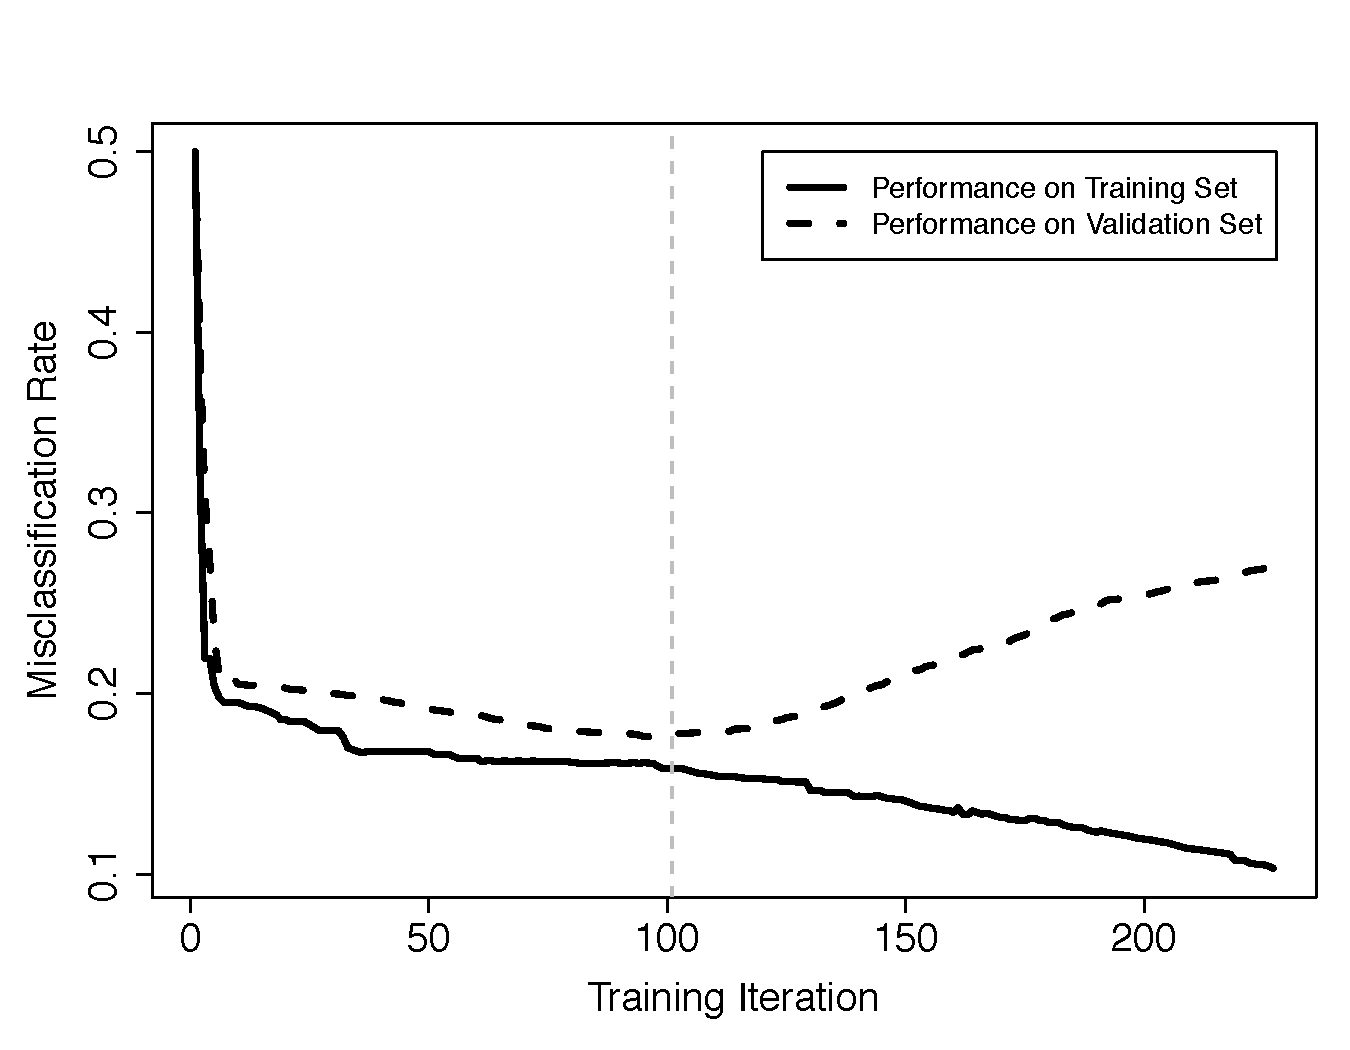
\includegraphics[width=0.54\linewidth]{images/InformationBased-ChurnIterationPlotRevised.pdf}
}
	\end{block}
\end{frame}

 \begin{frame} 
\begin{table}
\caption{An example validation set for the post-operative patient routing task.}
\label{tab:pruningset}
\centering
\begin{footnotesize}
\begin{tabular}{ c c c c c}
\hline
	 & \featN{Core-} & \featN{Stable-} &  & \\
\featN{ID}	 & \featN{Temp} & \featN{Temp} & \featN{Gender} & \featN{Decision}\\
\hline
1 & high & true & male & gen\\ 
2 & low & true & female & icu\\ 
3 & high & false & female & icu\\ 
4 & high & false & male & icu\\ 
5 & low & false & female & icu\\ 
6 & low & true & male & icu\\ 
\hline
\end{tabular}
\end{footnotesize}
\end{table}
\end{frame} 

 \begin{frame} 
\begin{figure}
\centerline{
	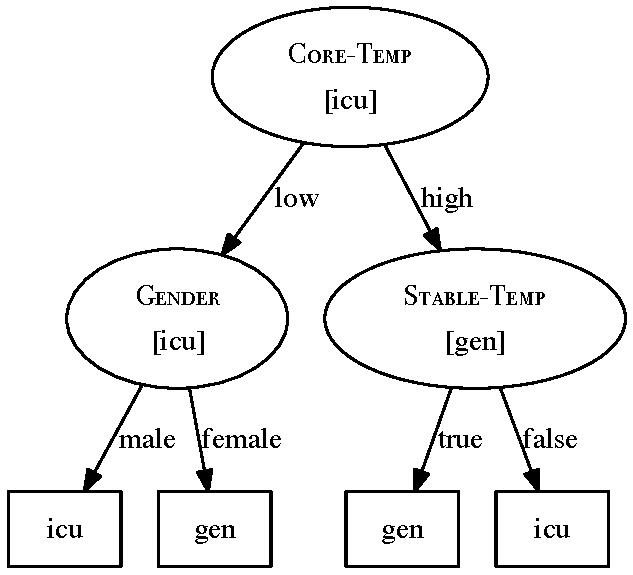
\includegraphics[width=0.4\textwidth]{./images/dtree-pruning-post-op1_mod.pdf}
}
\caption{The decision tree for the post-operative patient routing task.}
\label{fig:dtree-postop1}
\end{figure}
\end{frame} 


 \begin{frame} 
\begin{figure}
		\centering
\begin{footnotesize}
\begin{tabular}{ccc}
		\subfigure[]{\label{fig:errorpruning1} 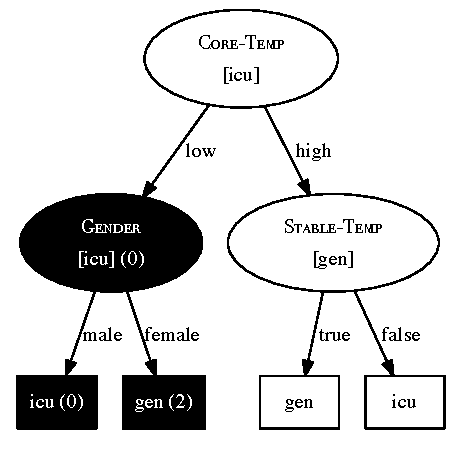
\includegraphics[width=0.33\linewidth]{./images/dtree-pruning-post-op2_mod.pdf}} &
		\subfigure[]{\label{fig:errorpruning2} 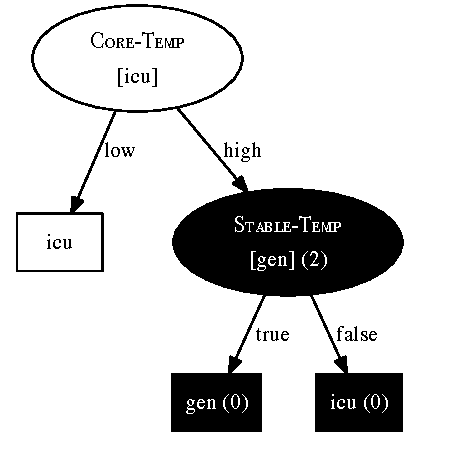
\includegraphics[width=0.31\linewidth]{./images/dtree-pruning-post-op3_mod.pdf}} &
		\subfigure[]{\label{fig:errorpruning3} 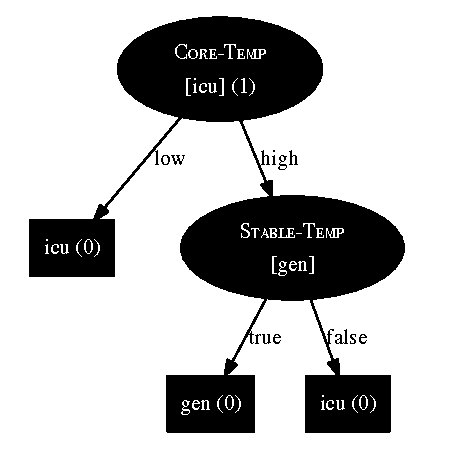
\includegraphics[width=0.31\linewidth]{./images/dtree-pruning-post-op4_mod.pdf}} \\
		\end{tabular}
\end{footnotesize}
	\caption{The iterations of reduced error pruning for the decision tree in Figure \ourRef{fig:dtree-postop1} using the validation set in Table \ourRef{tab:pruningset}. The subtree that is being considered for pruning in each iteration is highlighted in black. The prediction returned by each non-leaf node is listed in square brackets. The error rate for each node is given in round brackets.}
	\label{fig:errorpruning}
\end{figure}
\end{frame} 

\begin{frame}
Advantages of pruning:
\begin{itemize}
	\item Smaller trees are easier to interpret
	\item Increased generalization accuracy when there is noise in the training data (\keyword{noise dampening}). 
\end{itemize}
\end{frame}



\SectionSlideShortHeader{Model Ensembles}{Ensembles}

\begin{frame}
	\begin{itemize}
		\item Rather than creating a single model they generate a set of models and then make predictions by aggregating the outputs of these models. 
		\item A prediction model that is composed of a set of models is called a \keyword{model ensemble}.
		\item In order for this approach to work the models that are in the ensemble must be different from each other. 
	\end{itemize}
\end{frame}

\begin{frame}
	\begin{itemize}
		\item There are two standard approaches to creating ensembles:
		\begin{enumerate}
			\item \keyword{bagging}. 
			\item \keyword{boosting}
		\end{enumerate}
	\end{itemize}
\end{frame}

\subsection{Bagging}

 \begin{frame} 
	\begin{itemize}
		\item When we use \keyword{bagging} (or \keyword{bootstrap aggregating}) each model in the ensemble is trained on a random sample of the dataset known as \keyword{bootstrap samples}. 
		\item Each random sample is the same size as the dataset and \keyword{sampling with replacement} is used. 
		\item Consequently, every bootstrap sample will be missing some of the instances from the dataset so each bootstrap sample will be different and this means that models trained on different bootstrap samples will also be different
	\end{itemize}
\end{frame}

\begin{frame}
	\begin{itemize}
		\item When bagging is used with decision trees each bootstrap sample only uses a randomly selected subset of the descriptive features in the dataset. This is known as \keyword{subspace sampling}.
		\item The combination of bagging, subspace sampling, and decision trees is known as a \keyword{random forest} model.
	\end{itemize}
\end{frame} 


 \begin{frame} 
\begin{figure}[htb]
	\centering
	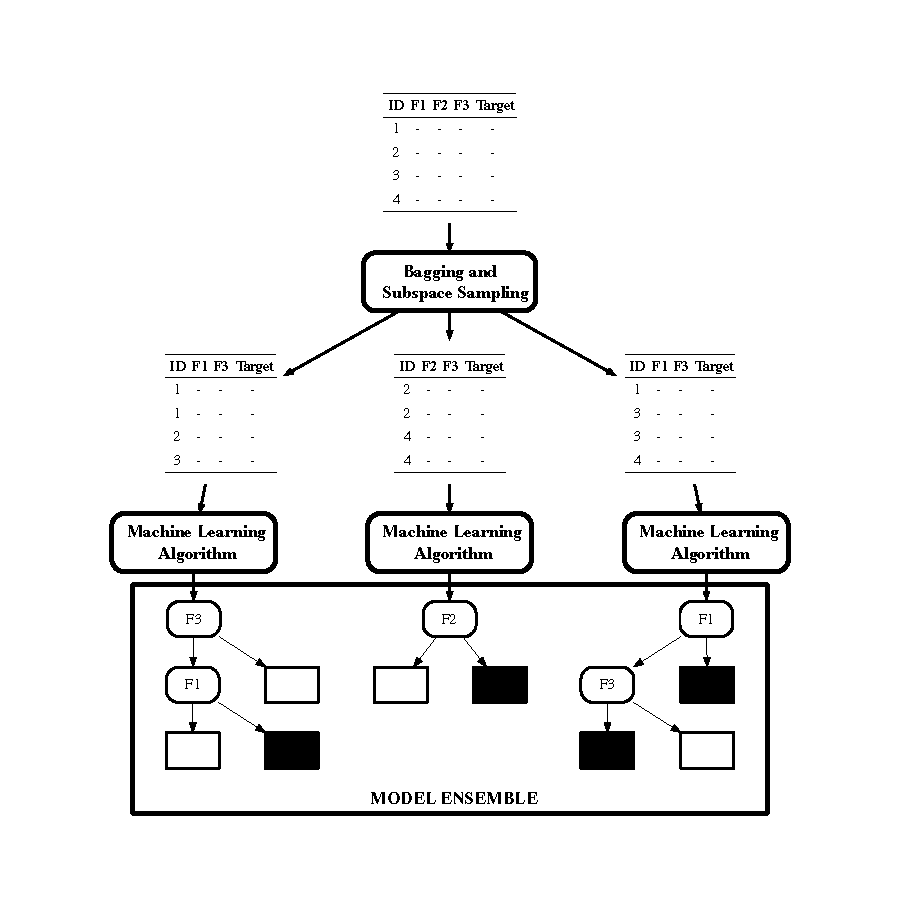
\includegraphics[width=0.5\textwidth]{./images/bagging.pdf}
	\caption{The process of creating a model ensemble using bagging and subspace sampling.}
	\label{fig:bagging}
\end{figure}
\end{frame} 


\subsection{Boosting}

\begin{frame}
\begin{itemize}
	\item Boosting works by iteratively creating models and adding them to the ensemble. 
	\item The iteration stops when a predefined number of models have been added.  
	\item When we use \keyword{boosting} each new model added to the ensemble is biased to pay more attention to instances that previous models miss-classified. 
	\item This is done by incrementally adapting the dataset used to train the models. To do this we use a \keyword{weighted dataset}
\end{itemize}
\end{frame}

\begin{frame}
	\begin{block}{Weighted Dataset}
		\begin{itemize}
			\item Each instance has an associated weight $\mathbf{w}_i\geq0$, 
			\item Initially set to $\frac{1}{n}$ where $n$ is the number of instances in the dataset. 
			\item After each model is added to the ensemble it is tested on the \alert{training data} and the weights of the instances the model gets correct are decreased and the weights of the instances the model gets incorrect are increased.
			\item These weights are used as a distribution over which the dataset is sampled to created a \alert{replicated training set}, where the replication of an instance is proportional to its weight.
		\end{itemize}
	\end{block}
\end{frame}

\begin{frame}
During each \alert{training iteration} the algorithm:
\begin{enumerate}
	\item Induces a model and calculates the total error, $\epsilon$, by summing the weights of the training instances for which the predictions made by the model are incorrect. 
	\item Increases the weights for the instances misclassified using:
\begin{equation}
	\mathbf{w}[i] \leftarrow \mathbf{w}[i] \times \left(\frac{1}{2 \times \epsilon}\right)
\end{equation}
\item Decreases the weights for the instances correctly classified:
\begin{equation}
	\mathbf{w}[i] \leftarrow \mathbf{w}[i]\times \left(\frac{1}{2 \times (1-\epsilon)}\right)
\end{equation}
	\item Calculate a \keyword{confidence factor}, $\alpha$, for the model such that $\alpha$ increases as $\epsilon$ decreases:
\begin{equation}
	\alpha = \frac{1}{2} \times log_e \left(\frac{1-\epsilon}{\epsilon}\right)
\end{equation}
\end{enumerate}
\end{frame}

\begin{frame}
\begin{itemize}
	\item Once the set of models have been created the ensemble makes \alert{predictions} using a weighted aggregate of the predictions made by the individual models. 
	\item The weights used in this aggregation are simply the confidence factors associated with each model. 
\end{itemize}
\end{frame}



 \begin{frame}
\begin{table}[!tb]
\caption{A simple bicycle demand predictions dataset and the workings of the first three iterations of training an ensemble model using boosting to predict \featN{Rentals} given \featN{Temp}.}
\label{tab:boost_demo_data}
\begin{scriptsize}
{\setlength{\tabcolsep}{0.1em}
\begin{tabular*}{26pc}{@{\extracolsep{\fill}}lrr rrr rrr rrr@{}}
\Toprule
~ &  ~ &  ~ & \multicolumn{3}{c}{Iteration 0} &  \multicolumn{3}{c}{Iteration 1}  &  \multicolumn{2}{c}{Iteration 2}  \\
\featN{ID} &  \featN{Temp} &  \featN{Rentals} & Dist. &  Freq. & $\mathbb{M}_{0}(\mathbf{d})$ &  Dist. &  Freq. & $\mathbb{M}_{1}(\mathbf{d})$ &  Dist. &  Freq. & $\mathbb{M}_{2}(\mathbf{d})$ \\
\Midrule
1  &            4 &     \featL{Low} &             0.100 &       2 &           \featL{Low} &           0.062 &       0 &          \featL{High} &           0.167 &       2 &           \featL{Low} \\
2  &            5 &     \featL{Low} &             0.100 &       1 &           \featL{Low} &           0.062 &       1 &          \featL{High} &           0.167 &       1 &           \featL{Low} \\
3  &            7 &     \featL{Low} &             0.100 &       0 &           \featL{Low} &           0.062 &       1 &          \featL{High} &           0.167 &       3 &           \featL{Low}\\
4  &           12 &    \featL{High} &             0.100 &       1 &          \featL{High} &           0.062 &       2 &          \featL{High} &           0.038 &       0 &           \featL{Low}\\
5  &           18 &    \featL{High} &             0.100 &       1 &          \featL{High} &           0.062 &       0 &          \featL{High} &           0.038 &       0 &           \featL{Low}\\
6  &           23 &    \featL{High} &             0.100 &       1 &          \featL{High} &           0.062 &       0 &          \featL{High} &           0.038 &       0 &           \featL{Low}\\
7  &           27 &    \featL{High} &             0.100 &       1 &          \featL{High} &           0.062 &       1 &          \featL{High} &           0.038 &       0 &           \featL{Low}\\
8  &           28 &    \featL{High} &             0.100 &       1 &          \featL{High} &           0.062 &       1 &          \featL{High} &           0.038 &       1 &           \featL{Low}\\
9  &           32 &     \featL{Low} &             0.100 &       2 &          \featL{High} &           0.250 &       3 &           \featL{Low} &           0.154 &       1 &           \featL{Low}\\
10 &           35 &     \featL{Low} &             0.100 &       0 &          \featL{High} &           0.250 &       1 &           \featL{Low} &           0.154 &       2 &           \featL{Low}\\
\Botrule
\end{tabular*}{}}
\end{scriptsize}
\end{table}
\end{frame} 



 \begin{frame} 
\begin{figure}[!tbh]
\begin{center}
{\setlength{\tabcolsep}{0.05em}
\begin{tabular}{cc}
		\subfigure[Training data]{\label{fig:boosting_bikes_demo_data}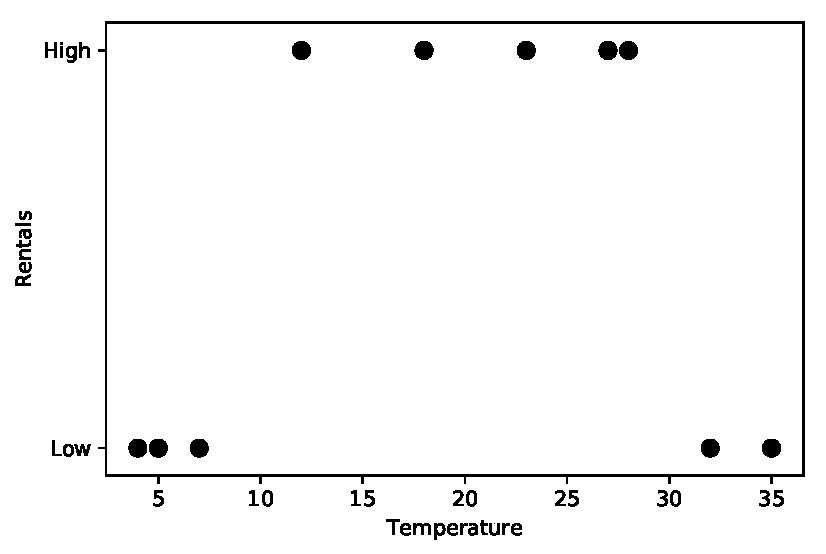
\includegraphics[width=0.48\linewidth]{./images/fmlpda_figure_4_21_a.pdf}} & \subfigure[The final ensemble model, $\mathbb{M}$]{\label{fig:boosting_bikes_demo_final}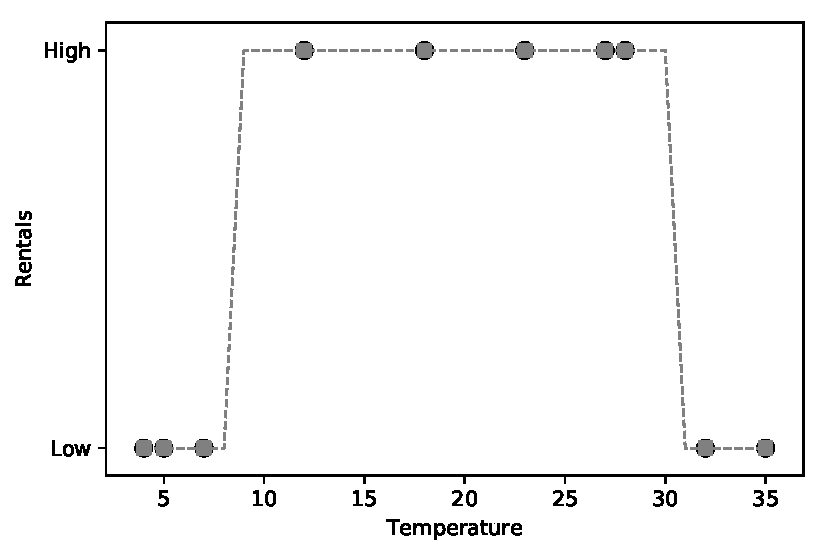
\includegraphics[width=0.48\linewidth]{./images/fmlpda_figure_4_21_b.pdf}} \\
\end{tabular}
}
\end{center}
\caption{(a) A plot of the bike rental dataset from Table \ourRef{tab:boost_demo_data}. (b) An illustration of the final ensemble model trained using the boosting algorithm. (c)--(e) A representation of the changing weights used to generate sample datasets for the first iterations of the boosting process.}
\label{fig:boosting_bikes_demo}
\end{figure}
\end{frame} 



 \begin{frame} 
\addtocounter{subfigure}{2}
\begin{figure}[!tbh]
\begin{center}
{\setlength{\tabcolsep}{0.05em}
\begin{tabular}{ccc}
		\subfigure[Distribution 0]{\label{fig:boosting_bikes_demo_dist_0}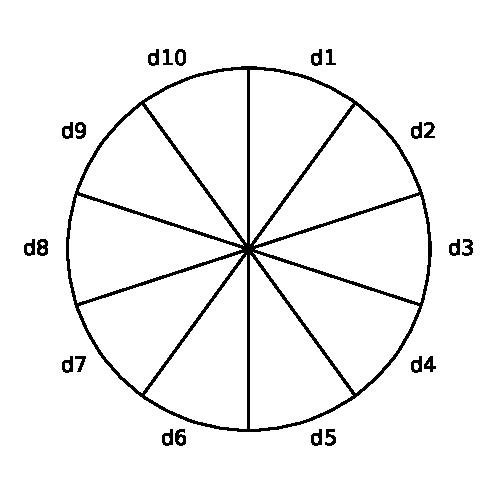
\includegraphics[width=0.333\linewidth]{./images/fmlpda_figure_4_21_c.pdf}} &
		\subfigure[Distribution 1]{\label{fig:boosting_bikes_demo_dist_1}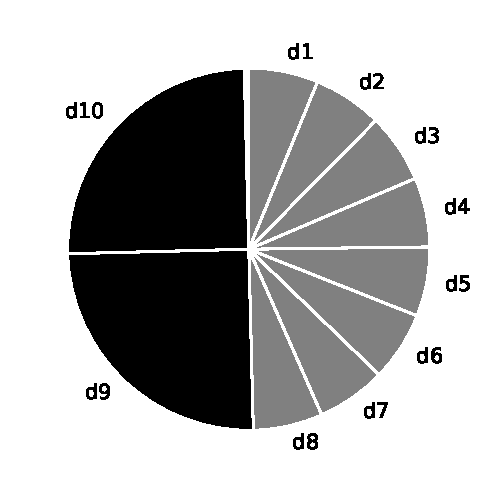
\includegraphics[width=0.333\linewidth]{./images/fmlpda_figure_4_21_d.pdf}} &
		\subfigure[Distribution 2]{\label{fig:boosting_bikes_demo_dist_2}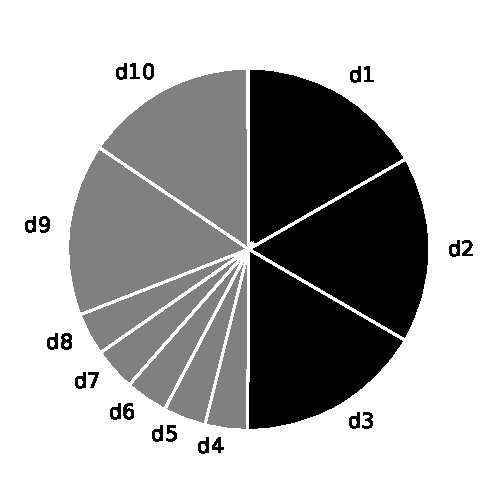
\includegraphics[width=0.333\linewidth]{./images/fmlpda_figure_4_21_e.pdf}} \\
\end{tabular}
}
\end{center}
\caption{(a) A plot of the bike rental dataset from Table \ourRef{tab:boost_demo_data}. (b) An illustration of the final ensemble model trained using the boosting algorithm. (c)--(e) A representation of the changing weights used to generate sample datasets for the first iterations of the boosting process.}
\label{fig:boosting_bikes_demo}
\end{figure}
\end{frame}


 \begin{frame} 
\begin{equation*}
\mathbf{w}\left[1\right] \leftarrow  0.100\times \left(\frac{1}{2 \times \left(1-0.200\right)}\right)   \leftarrow  0.0625  
\end{equation*}

~\\

\begin{equation*}
\mathbf{w}\left[9\right]  \leftarrow  0.100\times \left(\frac{1}{2 \times 0.200}\right)  \leftarrow 0.250 
\end{equation*}
\end{frame} 


\subsection{Gradient Boosting}


 \begin{frame} 
\begin{equation}
\mathbb{M}_{0}(\mathbf{d}) = \frac{1}{n}\sum_{i}t_i
\end{equation}

~\\

\begin{equation}
\mathbb{M}_{1}(\mathbf{d}) = \mathbb{M}_{0}(\mathbf{d}) + \mathbb{M}_{\Delta1}(\mathbf{d})
\label{eq:gb_first_iter}
\end{equation}

~\\

\begin{equation}
\mathbb{M}_{i}(\mathbf{d}) = \mathbb{M}_{i-1}(\mathbf{d}) + \mathbb{M}_{\Delta i}(\mathbf{d})
\label{eq:gb_recursion}
\end{equation}
\end{frame} 



 \begin{frame} 
\begin{alignat}{2}
\mathbb{M}_{4}(\mathbf{d}) & =  \mathbb{M}_{3}(\mathbf{d}) + \mathbb{M}_{\Delta 4}(\mathbf{d}) \nonumber \\
			 & = (\mathbb{M}_{2}(\mathbf{d}) + \mathbb{M}_{\Delta 3}(\mathbf{d})) + \mathbb{M}_{\Delta 4}(\mathbf{d}) \nonumber \\
			 & = ((\mathbb{M}_{1} + \mathbb{M}_{\Delta 2}(\mathbf{d})) + \mathbb{M}_{\Delta 3}(\mathbf{d})) + \mathbb{M}_{\Delta 4}(\mathbf{d})  \nonumber \\
			 & = (((\mathbb{M}_{0}(\mathbf{d}) + \mathbb{M}_{\Delta 1}(\mathbf{d})) + \mathbb{M}_{\Delta 2}(\mathbf{d})) + \mathbb{M}_{\Delta 3}(\mathbf{d})) + \mathbb{M}_{\Delta 4}(\mathbf{d}) \nonumber \\
			 & = \mathbb{M}_{0}(\mathbf{d}) + \mathbb{M}_{\Delta 1}(\mathbf{d}) + \mathbb{M}_{\Delta 2}(\mathbf{d}) + \mathbb{M}_{\Delta 3}(\mathbf{d}) + \mathbb{M}_{\Delta 4}(\mathbf{d})
\label{eq:gb_expansion}
\end{alignat}
\end{frame} 


\begin{frame}
\begin{table}
%\begin{adjustwidth}{-6pc}{-3pc}
\caption{A simple bicycle demand predictions dataset and the workings of the first iterations of training a gradient boosting model.}
\label{tab:grad_boost_demo_data}
\begin{tiny}
{\setlength{\tabcolsep}{0.1em}
\begin{tabular*}{27pc}{@{\extracolsep{\fill}}lrrrrrrrrrrrr@{}}
\Toprule
\featN{ID} &  \featN{Temp} &  \featN{Rentals} &  $\mathbb{M}_{0}(\mathbf{d})$ &  $t - \mathbb{M}_{0}(\mathbf{d})$ & $\mathbb{M}_{\Delta 1}(\mathbf{d})$  &  $\mathbb{M}_{1}(\mathbf{d})$ & $t - \mathbb{M}_{1}(\mathbf{d})$ & $\mathbb{M}_{\Delta 2}(\mathbf{d})$ &  $\mathbb{M}_{2}(\mathbf{d})$ &  $t - \mathbb{M}_{2}(\mathbf{d})$ &  $\mathbb{M}_{\Delta 3}(\mathbf{d})$ &  $\mathbb{M}_{3}(\mathbf{d})$ \\
\Midrule
1  &            4 &      602 &        1\,287.1 &      -685.1 &            -460.9 &       826.2 &    -224.2 &            -167.2 &       659.0 &     -57.0 &             -34.1 &       624.9 \\
2  &            5 &      750 &        1\,287.1 &      -537.1 &            -460.9 &       826.2 &     -76.2 &            -167.2 &       659.0 &      91.0 &             -34.1 &       624.9 \\
3  &            7 &      913 &        1\,287.1 &      -374.1 &            -460.9 &       826.2 &      86.8 &              71.6 &       897.8 &      15.2 &             -34.1 &       863.7 \\
4  &           12 &     1229 &        1\,287.1 &       -58.1 &            -460.9 &       826.2 &     402.8 &              71.6 &       897.8 &     331.2 &             -34.1 &       863.7 \\
5  &           18 &     1827 &        1\,287.1 &       539.9 &             691.4 &      1\,978.5 &    -151.5 &              71.6 &      2\,050.1 &    -223.1 &             -34.1 &      2\,016.1 \\
6  &           23 &     2246 &        1\,287.1 &       958.9 &             691.4 &      1\,978.5 &     267.5 &              71.6 &      2\,050.1 &     195.9 &             136.4 &      2\,186.5 \\
7  &           27 &     2127 &        1\,287.1 &       839.9 &             691.4 &      1\,978.5 &     148.5 &              71.6 &      2\,050.1 &      76.9 &             136.4 &      2\,186.5 \\
8  &           28 &     1714 &        1\,287.1 &       426.9 &             691.4 &      1\,978.5 &    -264.5 &              71.6 &      2\,050.1 &    -336.1 &             -34.1 &      2\,016.1 \\
9  &           32 &      838 &        1\,287.1 &      -449.1 &            -460.9 &       826.2 &      11.8 &              71.6 &       897.8 &     -59.8 &             -34.1 &       863.7 \\
10 &           35 &      625 &        1\,287.1 &      -662.1 &            -460.9 &       826.2 &    -201.2 &            -167.2 &       659.0 &     -34.0 &             -34.1 &       624.9 \\
\Botrule
\end{tabular*}{}}
\end{tiny}
%\end{adjustwidth}
%\end{table}
\end{table}
\end{frame}

 \begin{frame} 
\begin{figure}[tb]
\begin{center}
{\setlength{\tabcolsep}{0.05em}
\begin{tabular}[b]{cc}
	\subfigure[Training data]{\label{fig:gradient_boosting_bikes_demo_data}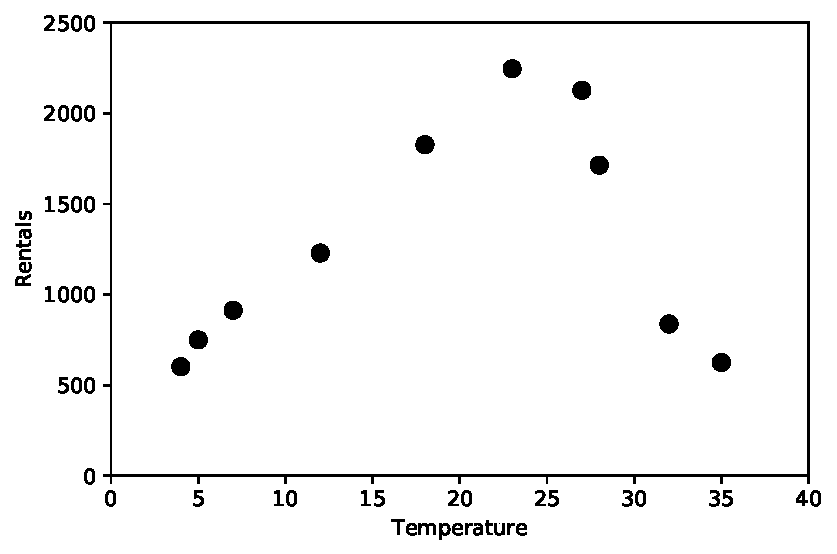
\includegraphics[width=0.42\linewidth]{./images/fmlpda_figure_4_22_a.pdf}} &
		\subfigure[$\mathbb{M}_{0}$]{\label{fig:gradient_boosting_bikes_demo_0}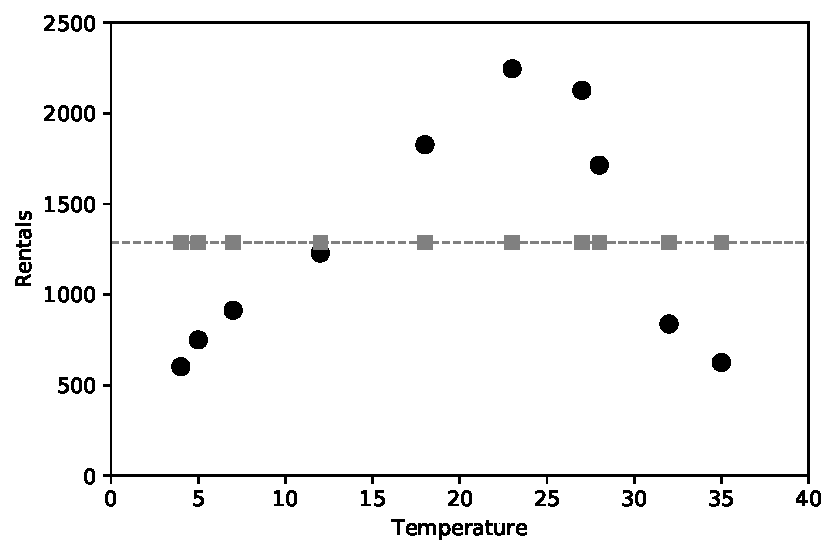
\includegraphics[width=0.42\linewidth]{./images/fmlpda_figure_4_22_b.pdf}} \\
\end{tabular}
}
\end{center}
\caption{(a) A plot of the bike rental dataset from Table \ourRef{tab:grad_boost_demo_data}. (b)--(e)  Visualizations of the prediction models trained in the early iterations of the gradient boosting process. (f) The final ensemble model trained after 20 iterations of gradient boosting.}
\label{fig:gradient_boosting_bikes_demo}

\end{figure}
\end{frame} 

 \begin{frame} 
 \addtocounter{subfigure}{2}
\begin{figure}[tb]
\begin{center}
{\setlength{\tabcolsep}{0.05em}
\begin{tabular}[b]{cc}
		\subfigure[$\mathbb{M}_{1}$]{\label{fig:gradient_boosting_bikes_demo_1}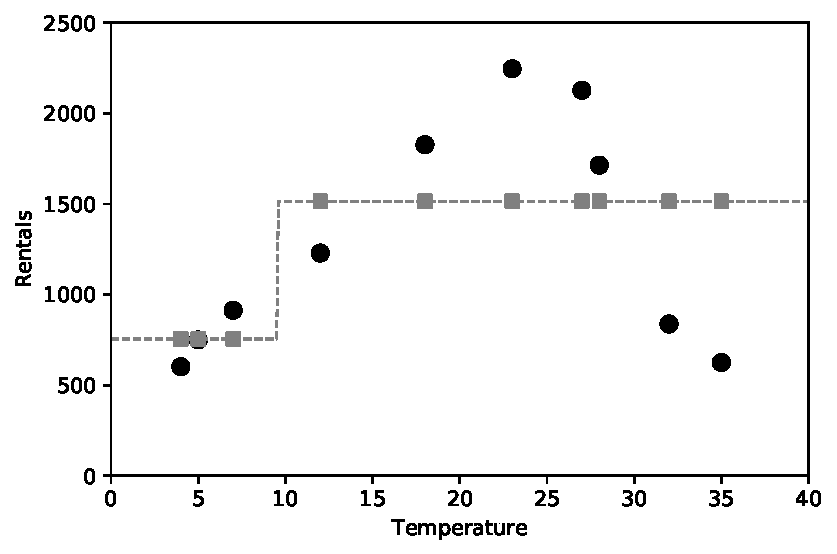
\includegraphics[width=0.42\linewidth]{./images/fmlpda_figure_4_22_c.pdf}} &
	\subfigure[$\mathbb{M}_{2}$]{\label{fig:gradient_boosting_bikes_demo_2}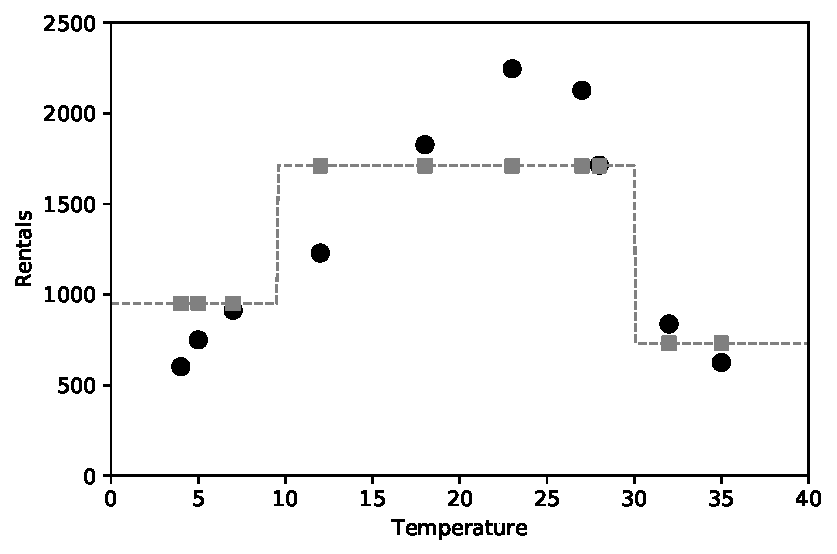
\includegraphics[width=0.42\linewidth]{./images/fmlpda_figure_4_22_d.pdf}} \\
\end{tabular}
}
\end{center}
\caption{(a) A plot of the bike rental dataset from Table \ourRef{tab:grad_boost_demo_data}. (b)--(e)  Visualizations of the prediction models trained in the early iterations of the gradient boosting process. (f) The final ensemble model trained after 20 iterations of gradient boosting.}
\label{fig:gradient_boosting_bikes_demo}

\end{figure}
\end{frame} 

 \begin{frame} 
  \addtocounter{subfigure}{4}
\begin{figure}[tb]
\begin{center}
{\setlength{\tabcolsep}{0.05em}
\begin{tabular}[b]{cc}
	\subfigure[$\mathbb{M}_{3}$]{\label{fig:gradient_boosting_bikes_demo_3}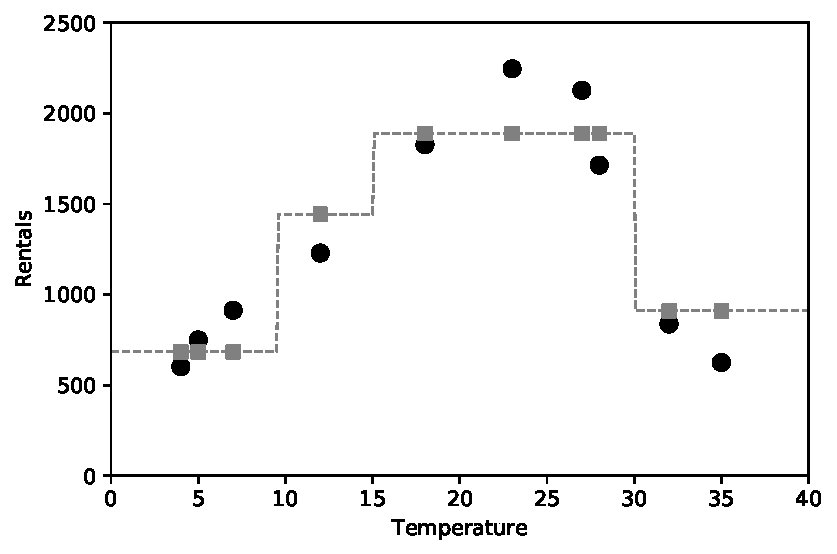
\includegraphics[width=0.42\linewidth]{./images/fmlpda_figure_4_22_e.pdf}} &
	\subfigure[$\mathbb{M}_{20}$]{\label{fig:gradient_boosting_bikes_demo_20}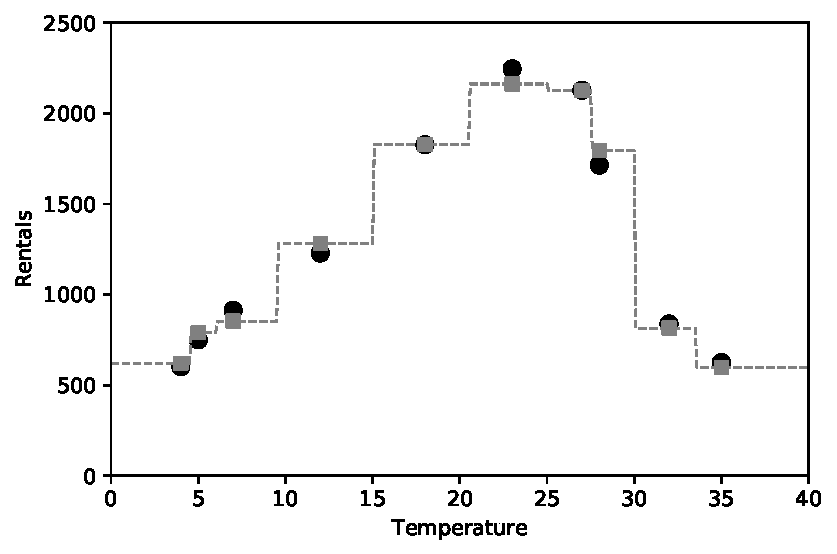
\includegraphics[width=0.42\linewidth]{./images/fmlpda_figure_4_22_f.pdf}} \\
\end{tabular}
}
\end{center}
\caption{(a) A plot of the bike rental dataset from Table \ourRef{tab:grad_boost_demo_data}. (b)--(e)  Visualizations of the prediction models trained in the early iterations of the gradient boosting process. (f) The final ensemble model trained after 20 iterations of gradient boosting.}
\label{fig:gradient_boosting_bikes_demo}

\end{figure}
\end{frame} 


 \begin{frame} 
\begin{equation}
\mathbb{M}_{i}(\mathbf{d}) = \mathbb{M}_{i-1}(\mathbf{d}) + \alpha \times \mathbb{M}_{\Delta i}(\mathbf{d})
\label{eq:gb_learning_rate}
\end{equation}
\end{frame} 




\begin{frame}
	\begin{itemize}
		\item Which approach should we use? Bagging is simpler to implement and parallelize than boosting and, so, may be better with respect to ease of use and training time. 
		\item Empirical results indicate:
		\begin{itemize}
			\item  boosted decision tree ensembles were the best performing model of those tested for datasets containing up to 4,000 descriptive features. 
			\item random forest ensembles (based on bagging) performed better for datasets containing more  that 4,000 features. 
		\end{itemize}
	\end{itemize}
\end{frame}

\SectionSlide{Summary}

\begin{frame}
	\begin{itemize}
		\item The \keyword{decision tree} model makes predictions based on sequences of tests on the descriptive feature values of a query 
		\item The \keyword{ID3} algorithm as a standard algorithm for inducing decision trees from a dataset. 
	\end{itemize}
\end{frame}

\begin{frame}
	\begin{block}{Decision Trees: Advantages}
		\begin{itemize}
			\item interpretable. 
			\item handle both categorical and continuous descriptive features. 
			\item has the ability to model the interactions between descriptive features (diminished if \keyword{pre-pruning} is employed) 
			\item relatively, robust to the \keyword{curse of dimensionality}.
			\item relatively, robust to noise in the dataset if \keyword{pruning} is used. 
		\end{itemize}
	\end{block}
\end{frame}

\begin{frame}
	\begin{block}{Decision Tress: Potential Disadvantages}
		\begin{itemize}
			\item trees become large when dealing with continuous features.
			\item decision trees are very expressive and sensitive to the dataset, as a result they can overfit the data if there are a lot of features (curse of dimensionality) 
			\item eager learner (concept drift). 
		\end{itemize}
	\end{block}
\end{frame}



\begin{frame}
	\tableofcontents
\end{frame}

\end{document}
